\documentclass[11pt, a4paper]{article}

%\usepackage{ngerman}
\usepackage[english]{babel}
\usepackage[utf8]{inputenc} %Korrekte Kodierung der Umlaute nach UTF-8
\usepackage[T1]{fontenc} %Korrekte Kodierung der Umlaute nach UTF-8
\usepackage{makeidx} %Zur automatischen Indexerstellung
\usepackage{amsfonts}
\usepackage{amssymb}
\usepackage{color}    % Verwendung von Farben
\usepackage{listings} % Korrekter Satz von Listings und Quellcode
\usepackage{tikz}     % graphen malen in latex
\usepackage{graphicx} % abbildungen einfügen
\usepackage{subfigure}
\usepackage{amsmath}  % mathe
\usepackage{amsthm}   % theoreme
\usepackage{footnote}
\usepackage{etoolbox} % common tools
\usepackage[colorlinks,
pdfpagelabels,
pdfstartview = FitH,
bookmarksopen = true,
bookmarksnumbered = true,
linkcolor = black,
urlcolor = black,
plainpages = false,
hypertexnames = false,
citecolor = black] {hyperref}
\usepackage{url}      % Korrekter Satz von URLs
% tkiz libs
\usetikzlibrary{calc,positioning,arrows,automata,decorations.pathreplacing,angles,quotes}


%Hilfs-Fonts - ohne Serifen (hier für Tabellen)
%\newfont{\bib}{cmss8 scaled 1040}
%\newfont{\bibf}{cmssbx8 scaled 1040}

% definitionen
\newtheorem{defi}{Defintion}
\newtheorem{theoreme}{Theorem}
\newtheorem{axiom}{Axiom}
\newcommand{\code}[1]{\texttt{#1}}

\definecolor{lightgray}{gray}{0.85}
\setlength{\emergencystretch}{1em} % erlaube zusätzliche abstände

\definecolor{codegreen}{rgb}{0,0.6,0}
\definecolor{codegray}{rgb}{0.5,0.5,0.5}
\definecolor{codepurple}{rgb}{0.58,0,0.82}
\definecolor{backcolour}{rgb}{0.95,0.95,0.92}

% define coq style
\lstdefinestyle{coq}{
  backgroundcolor=\color{backcolour},   
  commentstyle=\color{codegreen},
  keywordstyle=\color{magenta},
  numberstyle=\tiny\color{codegray},
  stringstyle=\color{codepurple},
  basicstyle=\ttfamily\footnotesize,
  breakatwhitespace=false,         
  breaklines=true,                 
  captionpos=b,                    
  keepspaces=true,                 
  numbers=left,                    
  numbersep=5pt,                  
  showspaces=false,                
  showstringspaces=false,
  showtabs=false,                  
  tabsize=2
}

%Seitenformat-Definitionen
\topmargin0mm
\textwidth147mm
\textheight214mm
\evensidemargin5mm
\oddsidemargin5mm
\footskip19mm
\parindent=0in

% \renewcommand{\lstlistingname}{Auflistung}
\apptocmd{\thebibliography}{\raggedright}{}{} % bibliography right aligned
\newcounter{sectionnumber}
\newcommand*\rot{\rotatebox{90}}

\makeindex % legt das Index-File an

\begin{document}          

\begin{titlepage}
  \begin{center} 
    \mbox{}
    
    {\large \sc Masterthesis} \\    

    \vspace{1cm}
  
    {\huge Implementing the RAFT consensus protocol with Velisarios in COQ\\[1em] {\LARGE}}  
        
    \vspace{2cm}
    
    
\includegraphics[scale=0.05]{images/Mathnatlogo.jpg}\\[1em]
    University of Potsdam\\
    Institute for Computer Science\\
    Professorship for theoretical Computer Science
    
    \vspace{2cm}
    
		submitted by
		
    \vspace{1em}
    
		{\Large Henrik Jürges} \\
        {Matr.-Nr. 751237}\\

    \vspace{2em}
        {Problem definition and supervision:}\\
        {Prof. Christoph Kreitz}\\
		
    \vspace{3em}    
    Potsdam\\
    30. March 2020
  \end{center}
\end{titlepage}


\pagenumbering{gobble}
% Zweite Seite = Kurzzusammenfassung
\begin{center}
{\bf Abstract}
\end{center}
\noindent

\newpage

% Dritte Seite = Inhaltsverzeichnis
\tableofcontents 
\newpage

\pagenumbering{Roman}
% Abkürzungsverzichnis
\newpage
\begin{appendix}
\section{Abkürzungen und Akronyme}\index{Akronyme}
\label{akro}
\begin{tabbing}
\hspace*{3cm}\=  \\ \kill
A2KB     \> Annotate to knowledge base\\
ASCII    \> American Standard Code for Information Interchange\\
C2KB     \> Concept to knowledge base\\
D2KB     \> Disambiguate to knowledge base\\
FTP      \> File Transfer Protocol\\
HITS     \> Hypertext-Induced Topic Search\\
HTML     \> Hypertext Markup Language\\
HTTP     \> Hypertext Transfer Protocol\\
IATA     \> International Air Transport Association\\
IE       \> Informationsextraktion\\
IEC      \> International Electrotechnical Commission\\
IRI      \> Internationalized Resource Identifiers\\
ISO      \> International Organization for Standardization\\
LOD      \> Linked Open Data\\
NED      \> Named Entity Disambigutation\\
NEL      \> Named Entity Linking\\
NEN      \> Named Entity Normalisation\\
NER      \> Named Entity Recognition\\
NIL      \> Not in List\\
NLP      \> Natural Language Processing\\
RDF      \> Resource Description Framework\\
RDFS     \> Resource Description Framework Schema\\
OWL      \> OWL 2 Web Ontology Language\\
SPARQL   \> SPARQL Protocol and RDF Query Language\\
URI      \> Uniform Resource Identifier\\
URL      \> Uniform Resource Locator\\
W3C      \> World Wide Web Community\\
WWW      \> World Wide Web\\
XML      \> Extensible Markup Language\\
\end{tabbing}
\newpage


\addcontentsline{toc}{section}{C~\,List of figures}
%\addcontentsline{toc}{section}{~~~~Abbildungsverzeichnis} % Zeile für das Inhaltsverzeichnis
\listoffigures

\newpage
\addcontentsline{toc}{section}{D~\,List of tables}
%\addcontentsline{toc}{section}{~~~~Tabellenverzeichnis} % Zeile für das Inhaltsverzeichnis
\listoftables
\end{appendix}
\newpage

\pagenumbering{arabic}
\setcounter{page}{1}
\setcounter{section}{0}
\renewcommand{\thesection}{\arabic{section}}
\newpage

\section{Einleitung}
\label{sec_einleitung}

% Motivation

 
\newpage
%
\section{Eventlogik}
\label{sec_logik}

%% einleitung %%
In diesem Kapitel wird die Eventlogik~\cite{bickford2003logic} nach Bickford und
Constable vorgestellt. Dazu werden die benötigten grundlegenden Logiken
und Theorien eingeführt.

%% grundlagen %%
\subsection{grundlegende Logiken}
% TODO
% Aussagenlogik
% Prädikatenlogik
% Logik 1. Ordnung
% dynamische Logik?
% Automatentheorie NEA

%% eventlogik %%
\subsection{Eventlogik}
Die Eventlogik nach Bickford und Constable baut auf der intuitunistischen Logik
auf. Sie verfolgt den ``correct-by-construction'' Ansatz, nach dem ein
funktionales Programm aus einem konstruktiven Beweis extrahiert werden kann.
Die Beweise haben die Grundform $\forall x:A.\exists : B.spec(x,y)$. Der konstruktive Beweis
liefert einen Extraktterm, der eine Realisierung des Beweises darstellt.
Da die Eventlogik die konstruktive Typentheorie benutzt sind alle
beweisbaren logischen Aussagen auch programmierbar, in dem Sinne, dass sie einen
Extraktterm besitzen der die Spezifikation erfüllt.~\cite{bickford2003logic}

% nachrichtenautomat
Grundlage für die Eventlogik ist ein Nachrichtenautomat. Dieser ist ein
nichtdeterministischer Automat der auf Nachrichten operiert.
Er hat die drei Basisoperationen ``senden'', ``empfangen'' und ``interne
Zustandsänderung''.~\cite{bickford2003logic}

\begin{defi}
  Ein Event $e=(a+m)$ ist ein Typ $A+M$ der entweder eine interne Aktion $A$ enthält
  oder eine empfangene Nachrichten $M$.
\end{defi}

\begin{defi}
  Ein Nachrichtenautomat ist ein abhängiger Datentyp mit der Struktur:
  $\{St, Act, Msg: Type, init: St$
    $f:(Act+Msg)\rightarrow St\rightarrow St$
    $send:(Act+Msg)\rightarrow St\rightarrow MsgList\}$  
\end{defi}

% verteilte Nachrichtenautomaten
Um verteilte Systeme darstellen zu können wird mehr als ein Nachrichtenautomat
benötigt, da ein Nachrichtenautomatenohne Interaktionen ein normaler
nichtdeterministischer Automat ist. Ein verteiltes System $V$ ist eine Menge von
Nachrichtenautomaten die in einem Netzwerk miteinander verknüpft sind.
Das Netzwerk ist fair, d.h. jede gesendete Nachricht wird auch unverändert
empfangen.~\cite{bickford2003logic}

\begin{defi}
  Ein verteiltes System $V$ ist ein Tupel $V=(M,L)$ wobei $m_i\in M$ mit $i\in
  \mathbb{N}$ die Menge der teilnehmenden Nachritenautomaten ist. $L$ beschreibt
  ein Kante in einem gerichteten Graphen und besteht aus dem Tupel $L=(s,d,m_i,m_j,Q)$ 
  mit $i,j\in \mathbb{N} und i \uneq j$. $Q$ ist eine Nachrichtenqueue.
\end{defi}





\newpage
%
\section{Practical Foundations}
\label{sec_3}

After the formal and logical foundations this chapter introduces
the practical aspects of building and using such a logic to build
reliable distributed systems is presented. This section covers Raft,
a bleeding-edge protocol to build distributed systems.
Afterward, a way to additionally harden such systems by using
the \textit{proofs-as-programs} approach is described.
This includes a short explanation of \textit{Coq} as well as
\textit{Velisarios} which is used to implement the \textit{Raft}
consensus protocol.

\subsection{Consensus Algorithms}
As mentioned in the introduction, distributed systems are useful to harden
critical infrastructures. A critical infrastructure is one where failures
of single components could lead to a disaster. So the information and
actions of single components shall be distributed and replicated to multiple
components holding the same state. The distributed system manages a
global state which is replicated over multiple members of the system and
a failure of some members can be tolerated. To harden the system further
the definition of failure is slightly different.~\cite{rahli2018velisarios}

\begin{defi}
  A byzantine failure is a failure which imposes no conditions.
\end{defi}

This means that a failure could happen at any time and the distributed
system has no reliable way to detect that a member failed or is malfunctioning.
Furthermore, a member could distribute false information across the network
and the system has to react reliably consistent to a certain limit of failures.~\cite{lamport1982byzantine}

\begin{defi}
  A typical byzantine fault-tolerant system can tolerate $n=3f+1$ failures
  where $n$ gives the number of members in the network to tolerate $f$ byzantine
  members.
\end{defi}

\begin{defi}
  A consensus protocol is an algorithm that allows a network of machines to
  agree on a common state of the network. The members act as a coherent
  group that could tolerate the failures of individual members.
\end{defi}

A consensus protocol is a state-of-the-art approach to build reliable and
resilient distributed systems that can tolerate byzantine failures.

\begin{figure}[ht]
  \centering
  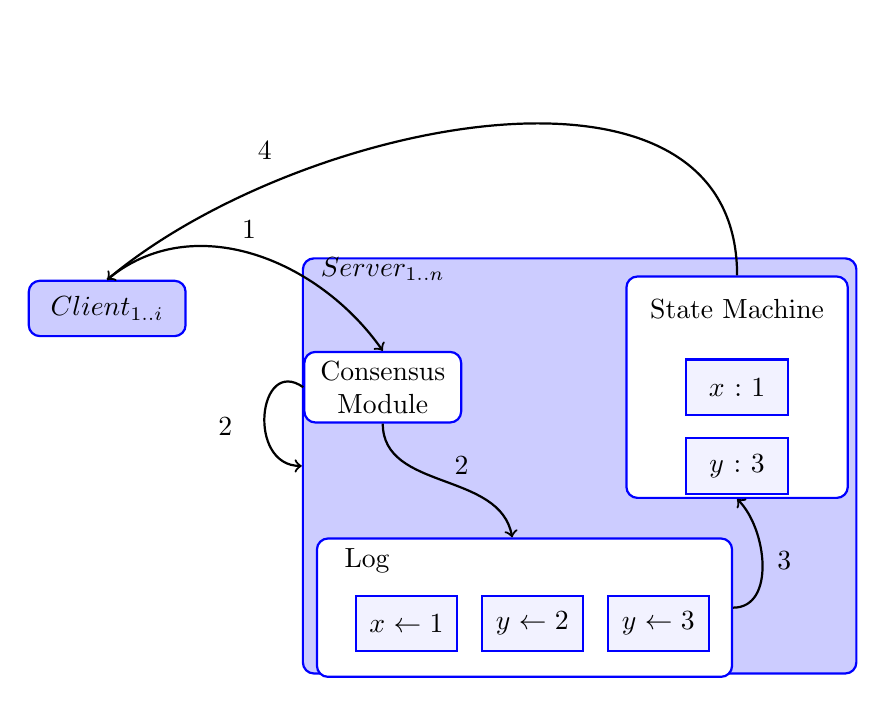
\begin{tikzpicture}[
    auto,
    block/.style={
      rectangle,
      draw=blue,
      thick,
      fill=blue!20,
      text width=5em,
      align=center,
      rounded corners,
      minimum height=2em
    }]

    % client box
    \draw (-6,2) node[block] (C) {$Client_{1..i}$};
    % server box
    \draw (0,0) node[
    block,
    minimum height=15em,
    minimum width=20em] (N) {};
    \node at (-2.5,2.5) {$Server_{1..n}$};
    % consensus
    \draw (-2.5,1) node[block,fill=white] (M) {Consensus Module};
    % log
    \draw (-0.7,-1.8) node[
    block,
    fill=white,
    minimum width=15em,
    minimum height=5em] (L) {};
    \node at (-2.7,-1.2) {Log};
    \draw (-2.2,-2) node[block,fill=blue!5,sharp corners,text width=3em] {$x\leftarrow 1$};
    \draw (-0.6,-2) node[block,fill=blue!5,sharp corners,text width=3em] {$y\leftarrow 2$};
    \draw (1,-2) node[block,fill=blue!5,sharp corners,text width=3em] {$y\leftarrow 3$};

    % state machine
    \draw (2,1) node[
    block,
    fill=white,
    minimum height=8em,
    minimum width=8em] (S) {};
    \node at (2,2) {State Machine};
    \draw (2,1) node[block,fill=blue!5,sharp corners,text width=3em] {$x: 1$};
    \draw (2,0) node[block,fill=blue!5,sharp corners,text width=3em] {$y: 3$};

    % lines
    \draw[->, thick] (C.north) to[out=40,in=125] (M.north) node at (-4.2,3) {1};
    \draw[->, thick] (M.south) to[out=-90,in=100] (L) node at (-1.5,0) {2};
    \draw[->, thick] (M.west) to[out=145,in=180,distance=2em] (N.west) node at (-4.5,0.5) {2};
    \draw[->, thick] (L.east) to[out=0,in=-45] (S.south) node at (2.6,-1.2) {3};
    \draw[->, thick] (S.north) to[out=90,in=40] (C.north) node at (-4,4) {4};
  \end{tikzpicture}
  \caption{Overview of the replicated state machine architecture.~\cite{ongaro2014search}}
  \label{fig:pbftsm}
\end{figure}

In figure~\ref{fig:pbftsm} an overview of the generic structures of the
replicated state machine architecture is presented. Most protocols using
replicated state machines act in the same manner. A possible bunch of clients
send their requests to the distributed network (1). The network can consist
of multiple servers. The consensus module is the middleware implementation of
the consensus protocol and acts as a mediator between the clients and servers.
The request is forwarded to all server consensus modules within the network (2).
Also the request is added to the server log. The request is seen as a command to
the server state machine and gets applied if the majority of the network
received the new command (3). Afterward, the client receives the result (4).
All server logs contain the same commands in the same order, so the servers
state machines process the commands in the same order and produce the same output.~\cite{ongaro2014search}

The major parts of the consensus algorithm are to ensure that the logs are
consistent across the servers, manage the client network communication,
handle the replication across the network and keep the network alive if
some server fails. So a consensus algorithm ensures the following properties:~\cite{ongaro2014search}

\begin{itemize}
\item Ensure safety under all non-byzantine conditions.
\item Ensure availability as long as the majority of servers are
  functional and can communicate.
\item Consistency doesn't depend on timing.
\item The system performance depends on the majority of servers
  and minorities can be ignored.
\end{itemize}

One early approach to build such distributed systems was presented by
Leslie Lamport et al as Paxos in~\cite{lamport1978time}.
Most of the newer protocols are directly derived from the early Paxos
protocol like~\cite{lamport2001paxos, van2015paxos}.
As Ongaro et al stated in~\cite{ongaro2014search} the family of
Paxos protocols suffer from two problems. Besides they ensure the
properties and provide an efficient protocol, the protocols are
difficult to understand. The descriptions are ``notoriously
opaque''~\cite{ongaro2014search} and are mostly focused on a
subset of the real world protocol. The other problem is that
most descriptions are not implementation ready and great effort
is needed to complete the missing parts of the protocol.
So, real-world implementations reflect the Paxos protocol only in
the beginning. To tackle these problems Ongaro et al made
the effort to design a new consensus protocol without the
Paxos history. This new protocol Raft was designed with
understandability in mind. This means, that the implementers'
effort needs to be minimized and the description and pseudo-code
needs to be as close to the real world as possible. Also,
the properties mentioned before need to be taken into account.
The resulting protocol shall be efficient and safe under
typical conditions and operations.~\cite{ongaro2014search}

\subsubsection*{The Raft protocol}
The algorithm is designed to manage a replicated log
across a distributed network. The protocol uses a leader-based
approach where one distinguished leader takes the full responsibility
for log replication and client handling. The other nodes are
only serving as dumb replicas. This approach
leads to three main components that can be viewed separately.~\cite{ongaro2014search}

\begin{itemize}
\item Leader election: Elect a new leader if the existing leader fails.
\item Log replication: The leader manages client requests and takes care
  of replicating his log across the network.
\item Safety:  The key property is the state machine safety which means that
  if any server has applied for a log entry no other server applies a
  different log entry at the same log index.
\end{itemize}

The last point is a set of five properties to ensure the liveness and
safety of the Raft protocol. The individual points are discussed at
their belongings.~\cite{ongaro2014search}

\begin{itemize}
\item Election safety: At all times at most one leader can be elected.
\item Leader Append-Only: New entries are only appended to the log and
  a leader never overwrites or deletes entries from its log.
\item Log Matching: If an entry is contained in two logs with the same
  term and index, these logs are identical up until the entries index.
\item Leader Completeness: If an entry is committed in some term, then the
  entry is present in all leader logs in all higher terms.
\item State Machine Safety: If a log entry with some index is applied to
  the internal state machine, then no other server ever applies a
  different log entry at the same index.
\end{itemize}

\paragraph{Basics}
A consensus protocol doesn't use real-time to measure the protocol progress
instead the time is divided into abstracts chunks of time. These chunks
serve as the logical clock of the protocol.~\cite{ongaro2014search}

\begin{defi}
  Time is divided into terms of arbitrary length where each term
  starts with an election phase which can be followed by a normal
  operation phase.
\end{defi}

This can be seen in figure~\ref{fig:terms}. The first term starts with an
election phase followed by a normal operation phase. The leader fails and
the term ends. The next term starts with an election phase which results in no
new leader and the next term is started.
Terms are numbered by consecutive integers and servers may observe term
transitions at different times. Each server stores its current term number
and exchanges it at every communication to detect failed leaders or outdated
data.~\cite{ongaro2014search}

\begin{figure}[ht]
  \centering
  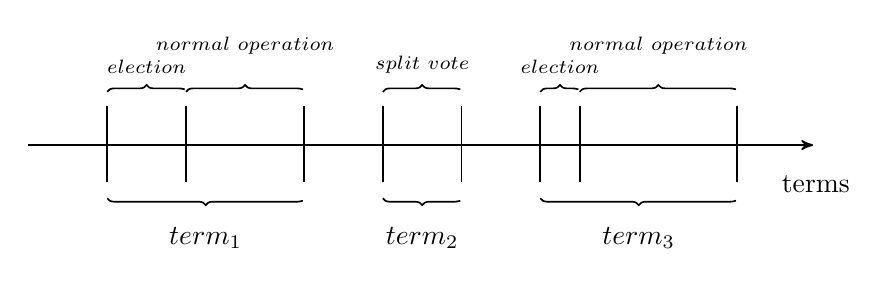
\begin{tikzpicture}[>=stealth',shorten >=1pt,auto,node distance=4cm,semithick]

    \draw[->] (-5,0) -- (5,0) node at (5,-0.5) {terms};
    % first term
    \draw (-4,0.5) -- (-4,-0.5);
    \draw (-3,0.5) -- (-3,-0.5);
    \draw (-1.5,0.5) -- (-1.5,-0.5);
    \draw[decoration={brace,mirror,raise=5pt},decorate] (-4,-0.5) -- node[below=12pt] {$term_1$} (-1.5,-0.5);
    \draw[decoration={brace,raise=5pt},decorate] (-4,0.5) -- node[above=8pt] {\scriptsize$election$} (-3,0.5);
    \draw[decoration={brace,raise=5pt},decorate] (-3,0.5) -- node[above=15pt] {\scriptsize$normal\ operation$} (-1.5,0.5);


    % second term
    \draw (-0.5,0.5) -- (-0.5,-0.5);
    \draw (0.5,0.5) -- (0.5,-0.5);
    \draw[decoration={brace,mirror,raise=5pt},decorate] (-0.5,-0.5) -- node[below=12pt] {$term_2$} (0.5,-0.5);
    \draw[decoration={brace,raise=5pt},decorate] (-0.5,0.5) -- node[above=8pt] {\scriptsize$split\ vote$} (0.5,0.5);

    %third term
    \draw (4,0.5) -- (4,-0.5);
    \draw (2,0.5) -- (2,-0.5);
    \draw (1.5,0.5) -- (1.5,-0.5);
    \draw[decoration={brace,mirror,raise=5pt},decorate] (1.5,-0.5) -- node[below=12pt] {$term_3$} (4,-0.5);
    \draw[decoration={brace,raise=5pt},decorate] (1.5,0.5) -- node[above=8pt] {\scriptsize$election$} (2,0.5);
    \draw[decoration={brace,raise=5pt},decorate] (2,0.5) -- node[above=15pt] {\scriptsize$normal\ operation$} (4,0.5);

  \end{tikzpicture}
  \caption{Example timeline within the protocol process.}
  \label{fig:terms}
\end{figure}

A server can be in one of three possible states at all times.
A server can either be a \textit{leader}, a \textit{follower}, or a
\textit{candidate}. Figure~\ref{fig:serverstates} shows the state
and the transition between them. Only one leader is allowed in normal operation
and all other servers are passive followers who obey the leaders' commands.
The followers aren't issuing requests on their own and only respond to requests
from the leader and candidates. The leader handles all client communication
and manages log replication across the followers. The candidate state is only
entered if the leader fails and a new leader needs to be elected.~\cite{ongaro2014search}

\begin{figure}[ht]
  \centering
  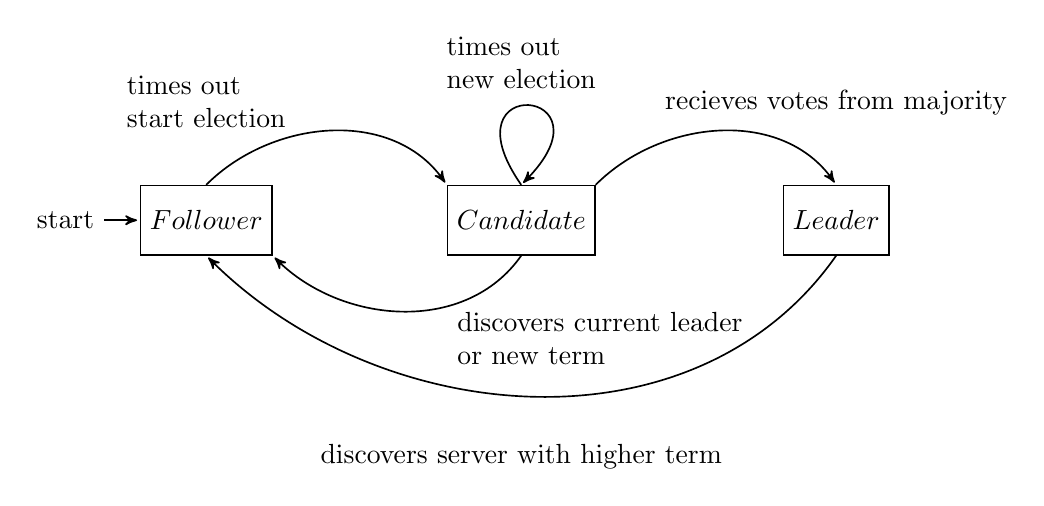
\begin{tikzpicture}[->,>=stealth',shorten >=1pt,auto,node distance=4cm,
    semithick]
    \tikzstyle{every state}=[rectangle]

    \node[initial,state] (A) {$Follower$};
    \node[state]         (B) [right of=A] {$Candidate$};
    \node[state]         (C) [right of=B] {$Leader$};

    \draw (A.north) to[out=45,in=125] (B.north west) node[align=left] at (0,1.5) {times out\\start election};
    \draw (B.north) to[out=125,in=45,distance=5em] (B.north) node[align=left] at (4,2) {times out\\new election};
    \draw (B.north east) to[out=45,in=125] (C.north) node[align=left] at (8,1.5) {recieves votes from majority};
    \draw (B.south) to[out=-125,in=-45] (A.south east) node[align=left] at (4,-3) {discovers server with higher term};
    \draw (C.south) to[out=-125,in=-45] (A.south) node[align=left] at (5,-1.5) {discovers current leader\\or new term};

  \end{tikzpicture}
  \caption{The server state transistions diagram.~\cite{ongaro2014search}}
  \label{fig:serverstates}
\end{figure}

\paragraph{Leader election}
As stated in figure~\ref{fig:serverstates} Raft uses timeouts to handle
leadership and election. Thus, every server has an internal timer with a
random time (mostly between 150 and 300ms) which gets reset with
every message from a leader. Besides normal messages the leader uses
heartbeat messages to reset the follower timers if the cluster is idle.
If a follower receives no messages over a while the
follower gets an \textit{election timeout}. It assumes the leader
failed and turns into a candidate state starting a new term and
election. The election runs as follows:~\cite{ongaro2014search}

\begin{enumerate}
\item A follower times out by receiving no messages over a while.
\item A follower increments its current term and turns into a candidate state.
\item A candidate votes for itself and issues the vote to the cluster.
\item Continue with point one until one of the following happens:
  \begin{enumerate}
  \item The candidate wins the election.
  \item Another candidate wins the election.
  \item The election times out with no winner.
  \end{enumerate}
\end{enumerate}

Since this may happen in parallel on many servers more details
need to be taken into account when determining the possible outcomes.

(a) A candidate wins the election when it receives the majority of
votes in the cluster. Each server votes for one candidate on a
\textit{first-come-first-serve} basis. The majority voting ensures
the only one leader safety property. The winner immediately starts
by sending heartbeat messages to all other servers to implement itself
as a new leader and stop the election phase.~\cite{ongaro2014consensus}\\
(b) A candidate may receive messages from a possible new leader.
The new leader is accepted if its term is at least as large as
the candidates one. The candidate accepts the new leader and turns
into a follower state. Otherwise, the leader is rejected and the election
goes on.~\cite{ongaro2014consensus}\\
(c) If multiple candidates start with the election at the same
time or the network connection is poor enough no candidate may win
the election. In this split vote scenario the candidate times out again
and starts a new term and election phase.\cite{ongaro2014consensus}

\paragraph{Log replication}
If a leader is elected the cluster transitions to the normal operation
state. This means that client requests are served, the requests are
replicated across the cluster and applied to the state machines.
The leader processes the client requests which contain commands to
the replicated state machine. The command is appended to the leaders
log as a new entry. Afterward, the leader issues replication requests
of this new entry to all other servers in parallel. If the majority
replicated the entry the leader commits the entry to its state machine
and responds the results to the client. The follower are noticed by
later messages of this newly committed entry. The leader
tries the replication of an entry indefinitely if some followers
are crashed or not responding.~\cite{ongaro2014search}

Figure~\ref{fig:logs} shows the organization of the logs of five servers,
one leader, and four followers. Each entry carries the command for the state
machine and the term number the entry was created to detect inconsistencies
between logs. Additionally, an entry is assigned to some log index number.
If an entry was safely replicated across the network and leader applies
it to its state machine, then the entry is committed and durable over
future terms. Also, the entry is eventually applied by all state machines
in the cluster. The leader tracks the highest known log index and includes
it in future requests such that followers know which entries can be
safely applied to their state machine. Previous entries that are
not already applied are then applied in log order.~\cite{ongaro2014consensus}

\begin{figure}[ht]
  \centering
  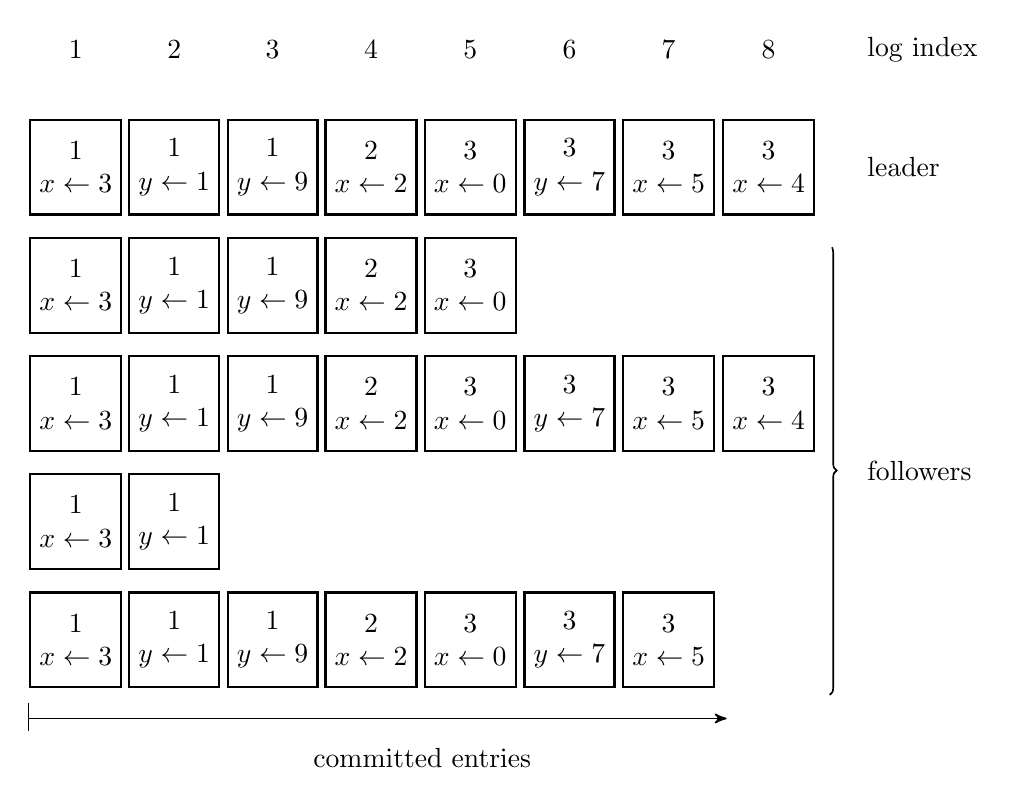
\begin{tikzpicture}[>=stealth',shorten >=1pt,auto,node distance=4cm,semithick]

    \draw[->] (-5,0) -- (3.9,0) node at (0,-0.5) {committed entries};
    \draw[-] (-5,0.2) -- (-5,-0.2);

    % first log
    \node at (-4.4,1) [draw,thick,rectangle,align=center,minimum height=1.2cm] {$1$\\$x\leftarrow 3$};
    \node at (-3.15,1) [draw,thick,rectangle,align=center,minimum height=1.2cm] {$1$\\$y\leftarrow 1$};
    \node at (-1.9,1) [draw,thick,rectangle,align=center,minimum height=1.2cm] {$1$\\$y\leftarrow 9$};
    \node at (-0.65,1) [draw,thick,rectangle,align=center,minimum height=1.2cm] {$2$\\$x\leftarrow 2$};
    \node at (0.61,1) [draw,thick,rectangle,align=center,minimum height=1.2cm] {$3$\\$x\leftarrow 0$};
    \node at (1.87,1) [draw,thick,rectangle,align=center,minimum height=1.2cm] {$3$\\$y\leftarrow 7$};
    \node at (3.13,1) [draw,thick,rectangle,align=center,minimum height=1.2cm] {$3$\\$x\leftarrow 5$};
    % second log
    \node at (-4.4,2.5) [draw,thick,rectangle,align=center,minimum height=1.2cm] {$1$\\$x\leftarrow 3$};
    \node at (-3.15,2.5) [draw,thick,rectangle,align=center,minimum height=1.2cm] {$1$\\$y\leftarrow 1$};
    % third log
    \node at (-4.4,4) [draw,thick,rectangle,align=center,minimum height=1.2cm] {$1$\\$x\leftarrow 3$};
    \node at (-3.15,4) [draw,thick,rectangle,align=center,minimum height=1.2cm] {$1$\\$y\leftarrow 1$};
    \node at (-1.9,4) [draw,thick,rectangle,align=center,minimum height=1.2cm] {$1$\\$y\leftarrow 9$};
    \node at (-0.65,4) [draw,thick,rectangle,align=center,minimum height=1.2cm] {$2$\\$x\leftarrow 2$};
    \node at (0.61,4) [draw,thick,rectangle,align=center,minimum height=1.2cm] {$3$\\$x\leftarrow 0$};
    \node at (1.87,4) [draw,thick,rectangle,align=center,minimum height=1.2cm] {$3$\\$y\leftarrow 7$};
    \node at (3.13,4) [draw,thick,rectangle,align=center,minimum height=1.2cm] {$3$\\$x\leftarrow 5$};
    \node at (4.4,4) [draw,thick,rectangle,align=center,minimum height=1.2cm] {$3$\\$x\leftarrow 4$};
    % fourth log
    \node at (-4.4,5.5) [draw,thick,rectangle,align=center,minimum height=1.2cm] {$1$\\$x\leftarrow 3$};
    \node at (-3.15,5.5) [draw,thick,rectangle,align=center,minimum height=1.2cm] {$1$\\$y\leftarrow 1$};
    \node at (-1.9,5.5) [draw,thick,rectangle,align=center,minimum height=1.2cm] {$1$\\$y\leftarrow 9$};
    \node at (-0.65,5.5) [draw,thick,rectangle,align=center,minimum height=1.2cm] {$2$\\$x\leftarrow 2$};
    \node at (0.61,5.5) [draw,thick,rectangle,align=center,minimum height=1.2cm] {$3$\\$x\leftarrow 0$};
    % fifth log
    \node at (-4.4,7) [draw,thick,rectangle,align=center,minimum height=1.2cm] {$1$\\$x\leftarrow 3$};
    \node at (-3.15,7) [draw,thick,rectangle,align=center,minimum height=1.2cm] {$1$\\$y\leftarrow 1$};
    \node at (-1.9,7) [draw,thick,rectangle,align=center,minimum height=1.2cm] {$1$\\$y\leftarrow 9$};
    \node at (-0.65,7) [draw,thick,rectangle,align=center,minimum height=1.2cm] {$2$\\$x\leftarrow 2$};
    \node at (0.61,7) [draw,thick,rectangle,align=center,minimum height=1.2cm] {$3$\\$x\leftarrow 0$};
    \node at (1.87,7) [draw,thick,rectangle,align=center,minimum height=1.2cm] {$3$\\$y\leftarrow 7$};
    \node at (3.13,7) [draw,thick,rectangle,align=center,minimum height=1.2cm] {$3$\\$x\leftarrow 5$};
    \node at (4.4,7) [draw,thick,rectangle,align=center,minimum height=1.2cm] {$3$\\$x\leftarrow 4$};
    
    \draw[decoration={brace,mirror,raise=5pt},decorate] (5,0.3) -- node[right=15pt] {followers} (5,6);
    \node at (5,7) [right=15pt] {leader};
    \node at (5,8.5) [right=15pt] {log index};
    \node at (-4.4,8.5) {1};
    \node at (-3.15,8.5) {2};
    \node at (-1.9,8.5) {3};
    \node at (-0.65,8.5) {4};
    \node at (0.61,8.5) {5};
    \node at (1.87,8.5) {6};
    \node at (3.13,8.5) {7};
    \node at (4.4,8.5) {8};
    
  \end{tikzpicture}
  \caption{An example of logs and its entries accross a cluster.~\cite{ongaro2014consensus}}
  \label{fig:logs}
\end{figure}

To maintain consistency between the logs Raft uses the aforementioned
log matching property which can be divided into two properties.

\begin{defi}
  If two entries have the same index and term in different logs, then
  they store the same command.
\end{defi}

\begin{defi}
  If two entries have the same index and term in different logs, then
  all preceding entries are identical in both logs.
\end{defi}

The leader organizes its log before distribution and logs stay
consistent over time. So, a leader doesn't change previous log index
entries and after distribution all other logs are coherent to the leaders
one. From this follows the first property. The second one follows
from the way an entry is replicated in the network. The leader
includes the previous entry term and index in the message. The follower only
applies the entry if it finds the given previous term and index in its
log. The consistency check preserves identical logs across the
network as long as no leader fails.~\cite{ongaro2014search}

If a leader crashes the log can become inconsistent through incomplete
replication. Also, this can be collected over multiple terms and
crashes of leaders and followers. A follower can have additional
or missing entries over multiple terms regarding the current leader.
The Raft approach to handle these inconsistencies are fairly simple.
The leader forces the followers to duplicate the leaders' log and
remove inconsistent entries from their logs. 
To do so, the leader maintains a list of the next log index
which is sent to a follower (initially the next empty log index of the leader). 
If the consistency check fails and the follower rejects to apply
an entry the leader decrements its next log index for the follower
and tries to replicate this entry. This happens until the leader
finds a matching entry in the follower log which removes all
succeeding entries and the leader can apply its log.~\cite{ongaro2014search}

\paragraph{Safety}
These mechanics doesn't ensure safety under all circumstances.
For example, if a leader is elected which has a shorter log
then the leader before the new leader may be remove already
committed entries from the network. This would break the
Leader Completeness property mentioned earlier. So, Raft
uses additional mechanics to ensure the correctness of
the safety properties.~\cite{ongaro2014search}

\subparagraph{Election restriction}
To prevent nodes with an incomplete log to be elected
Raft prevents candidates in the voting process from winning
the election. In the voting process a candidate messages
to at least a majority of other nodes in the network.
The messages contain the log index and term of the candidate
and the voter decides if the candidates log is up-to-date
enough to receive that vote.~\cite{ongaro2014search}

\begin{defi}
  Given two logs, the one is more up-to-date which has
  either the later term as last log entry or, if the terms
  are equal, the highest log index. Otherwise, both logs
  can be considered as equal.
\end{defi}

\subparagraph{Committing old entries}
If a leader crashes before committing an entry on the
majority of followers the new leader needs to handle
this situation by committing the entry. Raft never commits
log entries from previous terms by counting replicas and
checking if they are the majority. If a new entry is committed
to the majority of servers the leader applies the Log Matching
property to restore log consistency across the network.
Also, the log entries keep their term number and the
leader doesn't override the term number as with other
approaches. Thus, uncommitted log entries are only
committed indirectly by newer commits.~\cite{ongaro2014search}

\subparagraph{Follower and candidate failures}
Follower and candidate failures are fairly easy to handle.
Since all messages in Raft are idempotent the protocol
just resends all messages indefinitely until it gets
an expected result.~\cite{ongaro2014search}

\subparagraph{Client handling}
On startup, clients choose a random server for
requests. If the server is not the leader it rejects
the request with additional information about the current leader.
Otherwise, the network can implement internal forwarding of client
requests to the current leader. If the leader is unavailable the
requests time out.~\cite{ongaro2014consensus}

Raft supports linearizable semantics for clients. Each request
appears to be executed once and instantaneously. This is implemented
by assigning a unique id to every request. The network
caches every request along with the corresponding response preventing
it from re-executing old requests.~\cite{ongaro2014consensus}

\vspace{2em}

These are only the basics of the Raft algorithm which are implemented
in this thesis. Furthermore, Raft provides a description for log compaction,
cluster membership changes, and more further optimizations to the basic
algorithms. The next main section provides more details on the
implementation of the protocol within the Coq proofing system.

\subsection{Coq}
Coq is an interactive proof assistant that enables users to formalize
specifications and develop programs that fulfill these specifications.
These tools are developed for domains that require high standards in
the development and verification of programs. Also, it enables computer
scientists and mathematicians to develop proofs in an expressive
higher-order logic.~\cite{the_coq_development_team_2019_2554024}
The formalism used to provide such features is the \textit{Calculus of Inductive
  Construction}. It's a language that aims to represent functional programs
in an ML language style and proofs in higher-order logic (HOL).
It uses inductive definitions to represent data-structures, even infinite
ones. Based on the Curry-Howard-Isomorphism, Coq uses an approach based
on the \textit{Calculus of Construction} as a logical
background or metalanguage as described in the proofs-as-programs
sections.~\cite{the_coq_development_team_2019_2554024,
  paulinmohring:hal-01094195} This subsection gives only a brief overview
for a more comprehensive introduction use the reference documentation\footnote{\url{https://coq.inria.fr/refman/index.html}}.

The Calculus of Construction is an axiom-free typed polymorphic language.
The language of Coq allows us to define mathematical facts by
defining objects, like integers, sets, trees etc., and making statements
about the facts. By combining these one can write mathematical proofs.
The Coq compiler can automatically reason about the correctness of these
definitions and proofs by applying the rules of the type theory.
Additionally, Coq provides an environment to support the developer by
creating programs and proofs with various tools like proof search, advanced
notations, etc.~\cite{paulin2011introduction}

To enable this, Coq uses a small kernel language with only a few
primitive constructions, e.\,g. functions, (co-)inductive definitions,
product types, sorts. It is a pure and riched type $\lambda$-calculus that
describes terms and types.~\cite{paulinmohring:hal-01094195}.
It provides the basic $\lambda$ operations like binding, abstraction,
and application. Additionally, rules for type-checking and computation
are implemented on this level allowing the aforementioned reasoning
about the correctness.~\cite{paulin2011introduction, paulinmohring:hal-01094195}

The same language can be used to represent objects, functions, propositions,
and proofs that are on the higher-level. For this, Coq provides a
rich environment for designing theories, proofs, and programs. For instance,
this environment includes notations that are extensible, a tactic language,
a library system. These extensions are conservative and only safely extend the
basic kernel.~\cite{paulin2011introduction}

\begin{defi}
  Every Coq object or term has a name and a type.
\end{defi}

\begin{defi}
  Types are forming an infinite well-founded hierarchy.
  The type of types is called sort and the main sorts are:
  \begin{itemize}
  \item $Prop$ as the type of logical propositions.
  \item $SProp$ as the type of strict propositions.
  \item $Set$ as the type of small sets, for instance data types.
  \end{itemize}~\cite{the_coq_development_team_2019_2554024}
\end{defi}

\begin{defi}
  To support abstraction Coq uses \textbf{Definitions} to instantiate
  general statements with more concrete concepts used for proofs
  or programming.~\cite{huet1997coq}
\end{defi}

Definitions are one of the basic constructs which are used extensively
to define functions and facts about the program or theory.
Another important construct are inductive types which are used to model
data-types, primitive relations and so on in a constructive way.~\cite{paulin2011introduction}

\begin{defi}
  An inductive type declares a set of constructors that are used
  to construct every possible entity of the type. It introduces
  a new primitive object for the type and provides induction support
  on that type for reasoning.~\cite{paulin2011introduction}
\end{defi}

To use inductive types in functions or some other definitions Coq
uses \textit{pattern-matching} for case analysis over the type
constructors. It provides strong support for this by allowing
to match multiple patterns at once or by nesting patterns which
are also called \textit{generalized
  pattern-matching}.~\cite{paulin2011introduction}

The last important syntactical point mentioned here is the \textit{fixpoint definition}
which allows us to make recursive functions. To keep the logic sound, Coq uses
structural recursion instead of general recursion. This means that
such definitions use an inductive type as a formal argument.
Thus, on a recursive call the compiler can check that the next
term is structurally smaller than the previous one.~\cite{paulin2011introduction}

\paragraph{Extraction}
To use the logical and functional programs in the real world in conjunction
with other non-proven or type-checked languages, Coq offers
the possibility to extract formal code from Calculus of Inductive Construction.
Coq objects can be extracted into either Haskell or OCaml code and
some objects can also be exchanged by efficient ones from the target
language. This thesis extracts the code as OCaml library which can be
embedded in a command-line interface or simulation or evaluation
code for the Raft protocol.~\cite{the_coq_development_team_2019_2554024}

This is only a small overview of the possibilities Coq offers. Since
this thesis has no focus on building proofs, this part was skipped and
only the basic elements for building functional programs are shown to
understand the Velisarios framework in a basic way. Other constructs
are explained as they appear in the thesis.


\subsection{Velisarios}
This chapter shows the Raft protocols and the difficulties of
implementing distributed systems. The Logic of Events from the former
chapter shows a formal approach to handle these difficulties in
a consistent theory. It can tolerate byzantine failures and
imperfect information about the network. Rahli et al. presented
an implementation of the Logic of Events first in the NUPRL
theorem prover named EventML~\cite{rahli2017eventml}. Later
the system was reimplemented in Coq as Velisarios~\cite{rahli2018velisarios}.
It aims to be a generic and extensible formal verification framework
for developing and systematically proving distributed networks.~\cite{rahli2018velisarios}
%%
Schematically all byzantine fault-tolerant (BFT) protocols share the same
higher logic of distributing, gathering, and voting on the knowledge
provided to the system. Velisarios is a knowledge theory which
helps to build such systems by providing many main components
to reason about BFT protocols. For instance, a basic model
of the idea of arbitrary faults, a collection of assumptions
for reasoning, proof tactics and a general library of
knowledge of distributed systems.~\cite{rahli2018velisarios}

\begin{figure}[ht]
  \centering
  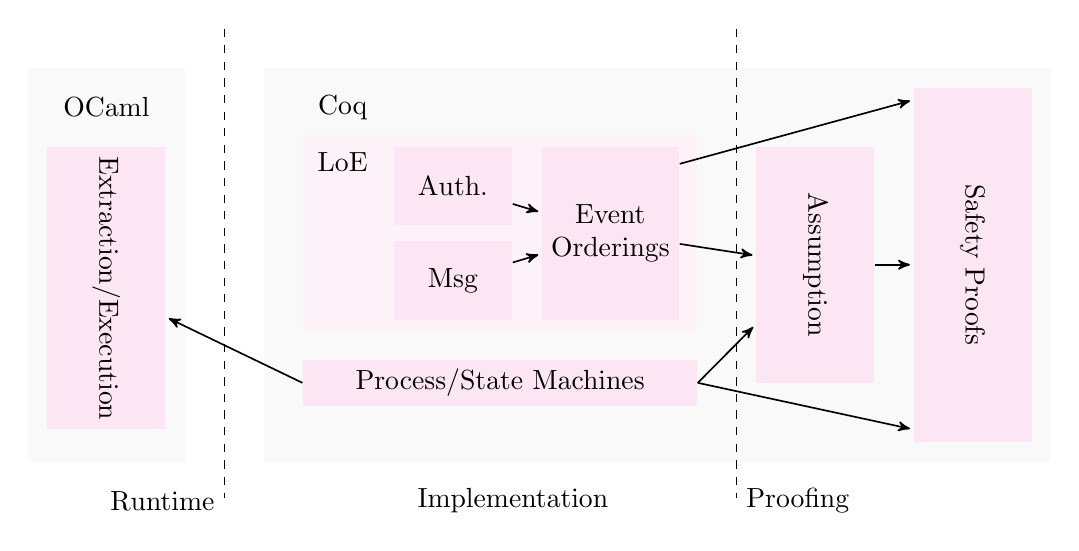
\begin{tikzpicture}[>=stealth',shorten >=1pt,auto, line width=1mm,semithick]

    % background layer
    \draw (0,0) node[rectangle, fill=gray!5, minimum width=10cm, minimum height=5cm] {};
    \draw (-7,0) node[rectangle, fill=gray!5, minimum width=2cm, minimum height=5cm] {};
    \draw (-7,2) node {OCaml};
    \draw (-4,2) node {Coq};

    % second layer
    \draw (-7,-0.3) node[rectangle, fill=magenta!10, rotate=-90, minimum height=1.5cm] (A) {Extraction/Execution};
    \draw (-2,0.4) node[rectangle, fill=magenta!5, minimum height=2.5cm, minimum width=5cm] {};
    \draw (-2,-1.5) node[rectangle, fill=magenta!10, minimum width=5cm] (B) {Process/State Machines};
    \draw (-4,1.3) node {LoE};
    \draw (2,0) node[rectangle, fill=magenta!10, rotate=-90, minimum height=1.5cm, minimum width=3cm] (C) {Assumption};
    \draw (4,0) node[rectangle, fill=magenta!10, rotate=-90, minimum height=1.5cm, minimum width=4.5cm] (D) {Safety Proofs};

    % top layer
    \draw (-2.6,1) node[rectangle, fill=magenta!10, minimum height=1cm, minimum width=1.5cm] (E) {Auth.};
    \draw (-2.6,-0.2) node[rectangle, fill=magenta!10, minimum height=1cm,minimum width=1.5cm] (F) {Msg};
    \draw (-0.6,0.4) node[rectangle, fill=magenta!10, align=center, minimum height=2.2cm] (G) {Event\\Orderings};

    % lines
    \draw[->] (B.west) -- (A);
    \draw[->] (E) -- (G);
    \draw[->] (F) -- (G);
    \draw[->] (B.east) -- (C);
    \draw[->] (G) -- (C);
    \draw[->] (G.45) -- (D.-160);
    \draw[->] (C) -- (D);
    \draw[->] (B.east) -- (D.-20);

    % parts
    \draw[dashed] (-5.5,3) -- (-5.5,-3) node [left] {Runtime};
    \draw[dashed] (1,3) -- (1,-3) node [left,xshift=-1.5cm] {Implementation}
    node [right] {Proofing};
    
  \end{tikzpicture}
  \caption{Overview of the Velisarios components.~\cite{rahli2018velisarios}}
  \label{fig:velisarios}
\end{figure}

As stated in the former chapter an event is an abstract entity that handles
received messages or reacts to some abstract activity which is no further
described. Velisarios use these arbitrary events to describe arbitrary faults.
A process reacts to messages happening at their locations one after another
by going through their states and creating new messages (which in turn
is a new event). Since events can be ordered by space and time a collection
of these events can be seen as a run of distributed systems. These are
called \textit{event orderings}. These orderings are the main idea when proving
properties about a distributed systems.~\cite{rahli2018velisarios}

\begin{defi}
  A property $P$ holds for a distributed system if it holds
  for all event orderings of that system.
\end{defi}

Figure~\ref{fig:velisarios} shows an overview of the components provided
by Velisarios. All components are abstract and parametrized to enable
reasoning and implementation of different protocols.~\cite{rahli2018velisarios}

As one can see, the core of Velisarios is the implementation of the Logic of
Events in terms of a message and authentication model which forms
the event orderings model.~\cite{rahli2018velisarios}

\paragraph*{Messages}
The messages are modeled as a type parameter \code{msg} of the overall model.
Processes react to incoming messages and may produce outgoing messages.
Messages are directed which hold the destination along with
the message and optional delay that holds the message back.~\cite{rahli2018velisarios}

\paragraph*{Destination}
A destination or node in the network has a type \code{name} which
identifies is in the network. The type belongs to the overall model.~\cite{rahli2018velisarios}

\paragraph*{Authentication}
Velisarios adds the abstract concept of keys for authenticated communication
to the overall model. A message can be authenticated by some nodes key
and the message can be checked for validity by some other node. The keys
are distinguished into sending and receiving ones that are preshared.
The model uses tokens to provide an abstraction for digital signatures.
The tokens are created by the appropriate sending key along with the data.
The receivers verify the correctness by checking that token with the receiving
key.~\cite{rahli2018velisarios}

These components form the event ordering component. It can be seen
as an abstract and formal representation of a run of a distributed system.
It is derived from the message sequence diagram used by most system designers.
The event orderings are no concrete type and are only used by Velisarios
to prove certain properties of the distributed system.~\cite{rahli2018velisarios}

\paragraph{Computational Model}
As shown below in the figure, Velisarios provides a process or state machine
model as a computational model for the logic of events. These state machines
are directly executable and the \code{name} of a node maps to the nodes
state machines. This enables the system to associate different state machines
to different nodes that can run independently.
The state machine is designed in a classical manner where
it consists of an initial state, a current state, and an update function
for state transitions as seen in Listing~\ref{lst:statemachines}.

\begin{lstlisting}[style=coq,float,label=lst:statemachines,caption=State
machine definition and update function.]
Definition Update S I O := S -> I -> (option S * O).
Record StateMachine S I O := 
  MkSM {halted : bool; update : Update S I O; state : S}.
Definition System (F : name -> Type) I O :=
  forall (i : name), StateMachine (F i) I O.
\end{lstlisting}

\code{S} is the type of the state machine and \code{I,O} are the input
and output types. The \code{halted} flag indicates if the particular
state machine is running or not. If an event \code{e} is received by
a state machine the local history of events is unrolled and
\code{state\_sm\_before\_event} creates the current state until
the new event. \code{state\_sm\_after\_event} updates the current
state by processing the messages of that event. Both functions
return \code{Some state} if an event is processed and otherwise
\code{None} if the state machines is halted or some error occurred.~\cite{rahli2018velisarios}

\paragraph{Extraction}
To evaluate and run the implemented protocol Velisarios
uses the Coq mechanics to extract OCaml code. Most of
the needed parameter is set as an extraction context beforehand
or only with stubs that get replaced by real implementations from
OCaml. the abstract parts, like event orderings, are not
instantiated and only used in Coq for proofing.~\cite{rahli2018velisarios}

\paragraph{Evaluation}
For the PBFT evaluation Rahli et al. build a small
trusted runtime in OCaml which uses the async library
\footnote{\url{https://opam.ocaml.org/packages/async/}}
for sending and receiving within threads. This system
is adapted by this thesis to match the Raft protocol.


%%% Local Variables:
%%% mode: latex
%%% TeX-master: "../master"
%%% End:

\newpage
%
\section{Inhaltliche Bestandteile der Seminararbeit}
\label{sec_inhalt}

\newpage
%
\section{Evaluation}
\label{sec_5}

The goal of this thesis was to implement the Raft protocol
with Velisarios. It should show that the programmers
effort to implement concensus protocols with COQ and
Velisarios are less error-prone and easier than other
approaches. Velisarios stands on a solid
logical foundation, the logic of events, and the
abstractions introduced by it narrow the effort
left for the implementors of distributed systems.
Additionally, COQ requires the programmer to rethink
its approach by providing only deterministic functions
and clean algebraic types. These restrictions and
the strong type-checking done by COQ lead to short and
precise functions. The functions are very predictive as they
act as mathematical functions with idempotence, so
a function returns the same outputs on the same inputs.

The strong distinction between state and functions operating
on that state which are only dependent types, lead to a
precise description of the protocol to implement.
The only failures that can happen are logical ones
in the COQ side of the code. The OCaml side is a little
bit different. Also, OCaml is a strong-typed language
it allows to ignore the type-checker and to mutate
types into different ones. This feature is heavily
used by the glue code to bridge the gap between
the COQ and OCaml type systems. This interface
can lead to all sorts of errors. These errors need
to be carefully traced because they originate in either
the COQ side or the OCaml side or both. So, an implementor
should write test cases for the main parts of the protocol
and verify the correctness of these. Maybe a verification
of the COQ code with Velisarios \code{EventOrderings}
can wipe out all failures on this side. But this part
was out of the reach of this thesis. 

Some parts of the description of Raft are not
obviously as expected. For example, the linearizable
semantics are a great concept and is described in a
detailed fashion but some points are left unsanswered.
The linearizable semantics are a key point to
prevent the global state machine to process requests
twice by using sessions for clients which are replicated
in the log. It uses a cache to respond to client requests
already processed but the concrete way of organizing
(either in the log or otherwise) and distributing of
the cache across the network are left to the readers
imagination. A more precise description of such things
can lead to a more comparable code base across the
different implementations since every different approach
has a great impact on the types and amount of messages
used. The core Raft only postulates four types
a messages but taken the case above into account a fifth
type is needed or not.

At a last point the tooling on the COQ side and the OCaml
side is not great. The COQ import facilities need a lot
of hand-craft to find the dependencies and work different
in the editor and the command-line. Upgrading the COQ
version can lead to broken builds and the need to adapt
the code to this specific version. On the OCaml side
the tooling is much better but requires the programmer
to craft and keep care of build files by themself.
A more elaborated tooling can substantial improve
the working and collaboration between the COQ and OCaml
ecosystems.

Because this thesis serves as a demonstration and
reference for future programmers a strong evaluation
based on benchmarking and comparison was not done.
A major reason was that only one other protocol
was already implemented with Velisarios which
has a greater implementation scope, for instance log compaction.
Also, other implementations of Raft didn't match this
state of implementation which makes it wrong to
compare them. This only leads to false assumptions
and conclusions about Raft. So, the evaluation
is only a recapitulation of the implementation process.


%%% Local Variables:
%%% mode: latex
%%% TeX-master: "../master"
%%% End:

\newpage
%
\section{Conclusion and Outlook}
\label{sec_conclusion}


\subsection{Conclusion}

This thesis showed the implementation of Raft using
Velisarios and the Logic of Events as a fundamental
basis for distributed consensus protocols. The Raft
thesis describes the protocol quite detailed and
straight foreward which makes the implementation
goes along with the description. Only some details
are left to the programmer to decide on how to implement
these parts and their interoperation. Also, many existing
implementations\footnote{\url{https://raft.github.io/}}
help to correctly interpret some not very clear points.
The diffculty with implementing something in COQ is that
it requires programmers from other languages or unfamiliar
with the functional concepts to rethink many parts
as other common languages are mostly based on an imperative
paradigm. Also, the
restriction to algebraic types and deterministic recursive
functions is not forseen by the description of Raft.
But these led to a more predictable and less error-prone
code so that mostly only logical failures are left as
bugs in the code. As shown with this thesis Velisarios
is a perfect fit for implementing distributed protocols
and using them in the real world. But one has to note that
Velisarios is addressed to programmers already familiar with the
concepts of \texttt{proofs-as-programs} and functional
programming in COQ and the tooling is far from perfect.
The basic aspects are described in the paper but the understanding about how the
parts fit together in code are left to the example
implementation of PBFT. In conclusion, this thesis
may serve as an additional reference point for
further approaches and implementions from non-theoretical
computer scientist.

\subsection{Outlook}

This thesis only showed the basic implementation of
Raft. There are a plethora of optimization points
and evaluation parts left. The original Raft paper
introduces membership changes in a cluster of nodes.
Since Velisarios does assumptions about the nodes
in the network beforehand and uses these assumptions
for the bijective representation of nodes and names
this feature can be quite tedious to implement.
Additionally, the Raft protocol provides log
compaction like most of the other Paxos protocols.
This can be easily integrated into the existing
implemntation by introducing a bunch of new message
types. With this feature the Raft protocol can be
compared to other protocols like the PBFT variant
implemented by the original Velisarios authors.
Also, the proving of the safety properties of
Raft is not done with the event orderings
introduced by Velisarios. With the proofs
done the implemented version of Raft
can be seen as a fully \texttt{proof-as-program}.
On a larger scale, more approaches to implement and
logical describe complex systems are needed. The
complexity of these system are hard to design
correctly by hand-woven code in non-functional
languages. So, these approaches maybe a common
standard in the future to handle complex systems
and make the life of programmers easier.



%%% Local Variables:
%%% mode: latex
%%% TeX-master: "../master"
%%% End:



\newpage
\begin{appendix}
\setcounter{section}{4}
\renewcommand{\thesection}{\Alph{section}}
\section{Glossar} %Appendix (Glossar)

Hier sollten die wichtigsten Schlüsselbegriffe, die in Ihrer Ausarbeitung thematisiert werden, knapp -- also wie in einem Lexikon -- gesammelt an einer Stelle zentral erläutert werden.
Das Glossar sollte im Umfang nicht mehr als eine Seite Ihrer Ausarbeitung einnehmen.
Sie müssen also allgemein bekannte Begriffe, wie z.B. \glqq Internet\grqq\, nicht unbedingt hier mit aufnehmen.

Die Erläuterung eines Begriffes im Glossar schließt nicht aus, dass Sie diesen Begriff bei seiner Einführung im Text nicht auch bereits erklärt haben. 


\begin{description}
\item[Browser:]\index{Browser} Ein spezielles Programm, mit dem man über das WWW Zugang zu WWW-Servern erlangen und von diesem angeforderte Dokumente anzeigen kann.

\item[Client:]\index{Client} Bezeichnet ein Programm, dass einen Server kontaktiert und von diesem Informationen anfordert. Der im WWW eingesetzte Browser ist in diesem Sinne ein Client. Aber es gibt auch andere Clients im WWW, die WWW-Server kontaktieren und Informationen von diesen herunterladen, wie z.B.~Suchmaschinen oder Agenten.

\item[HTML:]\index{HTML} Hypertext Markup Language; das einheitliche Dokumentenformat für Hyper\-media-Dokumente im WWW. Dokumente, die im WWW übertragen und vom Browser dargestellt werden sollen, sind in HTML kodiert.

\item[HTTP:]\index{HTTP} Hypertext Transfer Protocol; das Protokoll, das die Kommunikation von Browsern und WWW-Servern im WWW regelt. Fordert ein Browser ein Dokument vom WWW-Server an oder beantwortet der WWW-Server eine Anfrage, muss diese Anfrage den Konventionen des HTTP-Protokolls gehorchen. 

\item[Netzanwendung:]\index{Netzanwendungen} Ein Anwendungsprogramm, dessen Ablauf den Zugriff auf Ressourcen einschließt, die nicht lokal auf dem ausführenden Rechner\index{Rechner} liegen, sondern auf einem entfernten Rechner über das Netzwerk zugegriffen werden. 

\item[Server:]\index{Server} Bezeichnet einen Prozess\index{Prozess}, der von Clients kontaktiert wird, um diesen Informationen zurück zu liefern.
Oft wird auch der Rechner, auf dem ein Server-Prozess abläuft, als Server bezeichnet.
\end{description}


\newpage

% Appendix (Akronyme)
\section{Abkürzungen und Akronyme}\index{Akronyme}
Hier sollten {\bf alle} von Ihnen im Text verwendeten Abkürzungen in einem Verzeichnis zusammengestellt werden. 
Falls im Text keine Abkürzungen benutzt werden, brauchen Sie natürlich auch kein Abkürzungsverzeichnis zu erstellen.
\begin{tabbing}
\hspace*{3cm}\=  \\ \kill
4CIF \> 4 fach Common Intermediate Format\\
AAC \> Advanced Audio Coding\\
AAL \> ATM Adaption Layer\\
ABR \> Available Bit Rate\\
AC \> Audio Code\\
ACK \> Acknowledgement \\
ADM \> Add Drop Multiplexer\\
ADSL \> Asymmetric Digital Subscriber Line\\
AH \> Authentication Header\\
AIFF \> Audio Interchange File Format\\
AM \> Amplituden-Modulation\\
ANSI\> American National Standards Institute\\
API \> Application Programming Interface\\
ARP \> Address Resolution Protocol \\
W3C \> World Wide Web Community\\
WWW \> World Wide Web\\
\end{tabbing}

\end{appendix}

%Hier kommt das Literaturverzeichnis
\newpage
\addcontentsline{toc}{section}{~~~~Bibliography} % Zeile für das Inhaltsverzeichnis
\bibliography{bibfile}
\bibliographystyle{plain}

\newpage
%Hierhin kommt der Index (Sachverzeichnis)
%\addcontentsline{toc}{section}{Index} % Dies ist die Zeile für das Inhaltsverzeichnis
%\flushbottom                                    
%\printindex

\newpage
\section*{Selbstständigkeitserklärung}

Hiermit erkläre ich, Henrik Jürges, an Eides statt, dass ich die vorliegende Arbeit
"`Erweiterung des GERBIL-Frameworks zur Evaluation von Named-Entity-Linking Verfahren"'
selbstständig angefertigt, nicht anderweitig zu Prüfungszwecken vorgelegt und
keine anderen als die angegebenen Hilfsmittel verwendet habe. Sämtliche 
wissentlich verwendete Textausschnitte, Zitate oder Inhalte anderer Verfasser 
wurden ausdrücklich als solche gekennzeichnet und im Literaturverzeichnis aufgeführt.
\vspace{2mm}

Potsdam, den 29. April 2016
\vspace{4mm}

\newlength\us
\settowidth{\us}{-Henrik~Jürges-}
\begin{tabular}{p{\us}}\hline
\centering\footnotesize Henrik~Jürges
\end{tabular}

\end{document}

%%% Local Variables:
%%% mode: latex
%%% TeX-master: t
%%% End:
